\chapter{Polynomials}

\begin{definition}
    A Polynomial $P(x)$ is an one variable expression or function of the form
    \[
        P(x) = \sum_{i=0}^{n} a_{i}x^{i} = a_{n}x^{n} + a_{n-1}x^{n-1} + \cdots +a_{1}x + a_{0}
    \]
    where $a_{0},a_{1}, \cdots, a_{n}$ are constants and $n \in \mathbb{N}$. The constants $a_{i}$ are called the 
    \textit{coefficients} of the polynomial. We will denote $A[x]$ as the set of all polynomials with $a_{i} \in A$. If 
    $n\neq 0$ then $n$ is called the \textit{degree} of the polynomial $P(x)$ and write $\Deg P(x)=n$. 
    If $a_{n} = 1$ then we say that the polynomial is \textit{monic}. 
    $r$ is called a \textit{root} of the polynomial $P(x)$ if and only if $P(r)=0$.
\end{definition}

\section{Division Algorithm}

\begin{theorem}[The Division Algorithm]\label{thm:division-algorithm}
    Given two polynomial $A(x)$ and $B(x)$ there exists unique polynomials $Q(x)$ and $R(x)$ with $\Deg R(x) < \Deg B(x)$ 
    such that,
    \[
        A(x) = Q(x)B(x) + R(x)
    \]
    The polynomials $Q(x)$ and $R(x)$ are known as the \textit{quotient} and the \textit{remainder}, respectively. If the 
    remainder $R(x)=0$ then we say that $B(x)$ divides $A(x)$ and write $B(x) \mid A(x)$.
\end{theorem}
\begin{proof}
    We will first prove the uniqueness of the polynomials $Q(x)$ and $R(x)$. Assume,
    \begin{align*}
        & A(x) = Q_{1}(x)B(x) + R_{1}(x), \quad \Deg R_{1}(x) < \Deg B(x) \\
        & A(x) = Q_{2}(x)B(x) + R_{2}(x), \quad \Deg R_{2}(x) < \Deg B(x)
    \end{align*}
    Now,
    \begin{align*}
                 \left(Q_{1}(x) - Q_{2}(x)\right)B(x) + \left(R_{1}(x) - R_{2}(x)\right) = 0
    \end{align*}
    Let $q(x) = Q_{1}(x) - Q_{2}(x)$ and $r(x) = R_{1}(x) - R_{2}(x)$. Now,
    \begin{align*}
                 q(x)B(x) + r(x) = 0 \\
        \implies q(x)B(x) = -r(x)
    \end{align*}
    If $q(x)\neq 0$ then $\Deg r(x) = \Deg q(x) + \Deg B(x) \geq \Deg B(x)$. But that is impossible since 
    $\Deg R_{2}(x) < \Deg B(x) \implies \Deg \left(R_{2}(x) - R_{1}(x)\right) < \Deg B(x)$. Thus $q(x)$ must be zero. 
    Consequently $r(x)$ will also be zero. Therefore $R_{1}(x)=R_{2}(x)$ and $Q_{1}(x)=Q_{2}(x)$. \\
    Now we will prove the existence of the polynomials $Q(x)$ and $R(x)$. Notice the following algorithm,

    \begin{algorithmic}[1]
        \State $A(x) \gets a_{n}x^{n} + a_{n-1}x^{n-1}+\cdots+a_{0}$
        \State $B(x) \gets b_{n}x^{n} + b_{n-1}b^{n-1}+\cdots+b_{0}$
        \State $R(x) \gets A(x)$
        \While{$\Deg R(x) \geq \Deg B(x)$}
            \State $a \gets \text{leading coefficient of }R(x)$
            \State $b \gets \text{leading coefficient of }B(x)$
            \State $d \gets \Deg R(x) - \Deg B(x)$
            \State $Q(x) = Q(x) + \left(\frac{a}{b}\right)x^{d}$
            \State $R(x) \gets R(x) - \left(\frac{a}{b}\right)x^{d}B(x)$
        \EndWhile
        \Output $Q(x)$ and $R(x)$
    \end{algorithmic}
    In each iteration of the while loop, $\Deg R(x)$ is decreasing (mono-variant) and 
    the polynomial $Q(x)B(x) + R(x)$ always stays equal to $A(x)$ (invariant). 
    At some point we will eventually get $\Deg R(x) \leq \Deg B(x)$ which proves the existence of $Q(x)$ and $R(x)$.

    \begin{remark}
        Notice that, if $A(x), B(x) \in \mathbb{R}[x]$ then $Q(x), R(x) \in \mathbb{R}[x]$. This implies that, 
        if $A(x), B(x) \in \mathbb{R}[x]$ and $B(x)\mid A(x)$ then $\frac{A(x)}{B(x)} \in \mathbb{R}[x]$
    \end{remark}
\end{proof}

For example, if $B(x)= x^{2}-x+1$ and $A(x)=x^{5}+x^{3}+2x$ then,
\[
    x^{5}+x^{3}+2x = \left(x^{3}+x^{2}+x\right) \left(x^{2}-x+1\right) +x
\]
In this example, the remainder $R(x)=x$ and the quotient $Q(x)=x^{3}+x^{2}+x$. \\

\begin{theorem}[Remainder Theorem]\label{thm:remainder-theorem}
    If $P(x)$ is a polynomial and $a$ is a constant then the remainder upon dividing $P(x)$ by the linear 
    polynomial $x-a$ is equal to $P(a)$.
\end{theorem}
\begin{proof}
    From the \hyperref[thm:division-algorithm]{Division Algorithm} we know that there exists polynomials $Q(x)$ and $R(x)$ 
    such that,
    \[
        P(x) = Q(x)\left(x-a\right) + R(x)
    \]
    Since $\Deg R(x) < \Deg (x-a)=1$, $R(x)$ must be a constant polynomial. Let us assume, $R(x)=r$. 
    Now letting $x=a$ we get,
    \[
        P(a) = Q(a)\times (a-a) + r \implies P(a) = r
    \]
    Therefore $P(a)$ is the remainder upon dividing $P(x)$ by $x-a$. \textsf{QED}
\end{proof}

\begin{theorem}[Factor Theorem]\label{thm:factor-theorem}
    The number $z$ will be a root of the polynomial $P(x)$ if and only if $P(x)$ is divisible by $x-z$.
\end{theorem}
\begin{proof}
    We will first prove that, $P(z)=0 \implies (x-z) \mid P(x)$. 
    Let us assume that $r$ is the remainder upon dividing $P(x)$ by $x-z$. 
    Now we know from the \hyperref[thm:remainder-theorem]{Remainder Theorem} that, $P(z)=r$. 
    But since $z$ is a root of $P(x)$, $P(z)=r=0$. Therefore since $r=0$, we must have $(x-z)\mid P(x)$. 
    Using similar arguments one can also prove the converse. 
\end{proof}
\begin{corollary}
    The number $-\frac{b}{a}$ where $a, b\in \mathbb{R}$ will be a root of the polynomial $P(x)$ if and only if the 
    polynomial $P(x)$ is divisible by $ax+b$.
\end{corollary}

If $P(x)$ has the root $z$ then the \hyperref[thm:factor-theorem]{Factor Theorem} guarantees that there exists a polynomial 
$Q(x)$ such that,
\[
    P(x) = \left(x - z\right)Q(x)
\]
Now if,
\[
    P(x) = \left(x-z\right)^{m}Q'(x), \quad Q'(z) \neq 0
\]
then we say that $z$ is root of $P(x)$ of \textit{multiplicity} $m$. \\
For example, in the polynomial $P(x)=\left(x-2\right)^{2}\left(x-3\right)$ 
the root 2 has multiplicity 2 and the root 3 has multiplicity 1.

\section{The Fundamental Theorem of Algebra}

\begin{theorem}[The Fundamental Theorem of Algebra]\label{thm:fta}
    The Fundamental Theorem of Algebra states that, every polynomial $P(x)$ in $\mathbb{C}[x]$ has at least 
    one root in $\mathbb{C}$
\end{theorem}
\begin{corollary}
    If $P(x) = a_{n}x^{n} + a_{n-1}x^{n-1} + \cdots + a_{1}x + a_{0}$ is a polynomial of degree $n$ then,
    \[
        P(x) = k(x - z_{1})(x - z_{2})\cdots (x - z_{n})
    \]
    where, $k = a_{n}$ and $z_{i} \in \mathbb{C}$. The numbers $z_{1},z_{2}\cdots z_{n}$ are not necessarily 
    distinct.
\end{corollary}
\begin{proof}
    This is an immediate consequence of \hyperref[thm:fta]{The Fundamental Theorem of Algebra} 
    and \hyperref[thm:factor-theorem]{Factor Theorem}.
\end{proof}

\begin{figure}[!htpb]
\centering
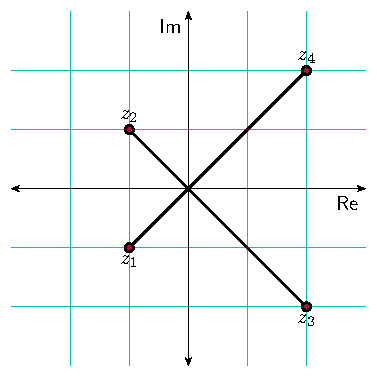
\includegraphics[scale=1]{polynomials/figures/cplane_roots.pdf}
\caption{The 4 complex roots of the polynomial $x^{4} - 2 x^{3} + 2 x^{2} + 8 x + 16$ }
\label{fig:cplane_roots}
\end{figure}

\begin{theorem}[Complex Conjugate Root Theorem]
    If $P(x) \in \mathbb{R}[x]$ and $z=a+bi$ where $a,b \in \mathbb{R}$ is a complex root of the polynomial 
    $P(x)$ then $\overline{z}=a-bi$ is also a root of the polynomial $P(x)$.
\end{theorem}
\begin{proof}[1]
    We have to show that, $P(z)=0 \implies P(\overline{z})=0$. Let $\mathbb{C}'=\left\{ki:k\in\mathbb{R}\right\}$ and let 
    $\mathbb{R}$ be the set of real numbers. Now,
    \begin{align*}
        z^{k} + \overline{z}^{k} &= (a+bi)^{k} + (a-bi)^{k} \\
                                 &= 
                                  \sum_{j=0}^{k} {k \choose j} b^{j} a^{k-j} i^{j} +
                                  \sum_{j=0}^{k} {k \choose j} b^{j}a^{k-j} (-i)^{j} \\
                                 &=
                                 \sum_{j=0}^{k} {k \choose j} b^{j} a^{k-j} \left\{i^{j} + (-i)^{j} 
                                 \right\}
    \end{align*}
    Notice, $i^{j} + (-i)^{j}$ will be zero if $j$ is odd. If $j$ is even then $i^{j} + (-i)^{j} = 2i^{j} = 2(-1)^{\frac{j}{2}}$. 
    Therefore,
    \begin{align*}
        z^{k} + \overline{z}^{k} &= 
                                 \sum_{j=0}^{k} {k \choose j} b^{j} a^{k-j} \left\{i^{j} + (-i)^{j} 
                                 \right\} \\ 
                                 &=
                                 \sum_{l=0}^{\floor{\frac{k}{2}}} {k \choose 2l} b^{2l} a^{k-2l}
                                 \left\{2(-1)^{l}\right\}\\
                                 &= \sum_{l=0}^{\floor{\frac{k}{2}}} {k \choose 2l} 2(-1)^{l} b^{2l} a^{k-2l}
    \end{align*}
    \begin{remark}
        The set, $\left\{ 2l : 0 \leq l \leq \floor{\frac{k}{2}}\right\}$, contains all even integers (including zero) less than 
        or equal to $k$.
    \end{remark}
    Therefore, $z^{k} + \overline{z}^{k} \in \mathbb{R}$ for all $0\leq k\in \mathbb{Z}$. This implies that,
    \begin{equation*}
        P(z) + P(\overline{z}) = \sum_{i=0}^{n} a_{i} \left( z^{i} + \overline{z}^{i} \right) \in \mathbb{R} 
    \end{equation*}
    But since $P(z)=0$, $P(z) + P(\overline{z}) \in \mathbb{R}$ implies $P(\overline{z})\in \mathbb{R}$. Now,
    \begin{align*}
        z^{k} - \overline{z}^{k} &= (a+bi)^{k} - (a-bi)^{k} \\
                                 &= 
                                  \sum_{j=0}^{k} {k \choose j} b^{j}a^{k-j} i^{j} -
                                  \sum_{j=0}^{k} {k \choose j} b^{j}a^{k-j} (-i)^{j} \\
                                 &=
                                 \sum_{j=0}^{k} {k \choose j} b^{j}a^{k-j}
                                 \left\{i^{j} - (-i)^{j}\right\}
    \end{align*}
    If $j$ is even then $i^{j} - (-i)^{j}$ will be equal to zero. If $j$ is odd that is $j=2l-1$ for some $l\in \mathbb{N}$ then 
    $i^{j} - (-i)^{j} = i^{2l-1} \left( 1 - (-1)^{2l-1} \right)=2i^{2l-1} = 2(-1)^{l}i^{-1} = 2(-1)^{l}i^{3} = 2(-1)^{l+1}i$. \\
    Therefore,
    \begin{align*}
        z^{k} - \overline{z}^{k} &= 
                                 \sum_{j=0}^{k} {k \choose j} b^{j}a^{k-j}
                                 \left\{i^{j} - (-i)^{j}\right\} \\
                                 &=
                                 \sum_{l=1}^{\floor{\frac{k+1}{2}}} 
                                 {k \choose 2l-1} b^{2l-1}a^{k-2l+1} 2(-1)^{l+1}i \\
                                 &= 
                                 \left( \sum_{l=1}^{\floor{\frac{k+1}{2}}}
                                 {k \choose 2l-1} b^{2l-1}a^{k-2l+1} 2(-1)^{l+1}\right)i
    \end{align*}
    \begin{remark}
        The set $\left\{2l-1: 1\leq l \leq \floor{\frac{k+1}{2}}\right\}$ contains all odd positive integers less than or equal 
        to $k$.
    \end{remark}
    Thus, $z^{k} - \overline{z}^{k}\in \mathbb{C}'$ for all $k\in \mathbb{N}$. Now,
    \begin{align*}
        P(z) - P(\overline{z}) &= \sum_{i=0}^{n} a_{i} \left( z^{i} - \overline{z}^{i} \right)\\
        \implies P(z) - P(\overline{z}) &= \sum_{i=1}^{n} a_{i} \left( z^{i} - \overline{z}^{i} \right) 
                               + a_{0}\left( z^{0} - \overline{z}^{0} \right) \\
        \implies P(z) - P(\overline{z}) &= \sum_{i=1}^{n} a_{i} \left( z^{i} - \overline{z}^{i} \right) \in \mathbb{C}'
    \end{align*}
    But since $P(z)=0$, $P(z) - P(\overline{z}) \in \mathbb{C}'$ implies $P(\overline{z}) \in \mathbb{C}'$. And so, 
    $P(\overline{z})\in \mathbb{R} \cup \mathbb{C}' \implies P(\overline{z}) \in \{0\} \implies P(\overline{z}) = 0$. 
    \textsf{QED}
\end{proof}
\begin{proof}[2(wiki)]
    Since $P(z)=0$,
    \begin{equation*}
        P(z) = \sum_{k=0}^{n} a_{k} z^{k} = 0
    \end{equation*}
    Now using the properties of complex conjugates,
    \begin{align*}
        P(\overline{z}) = \sum_{k=0}^{n} a_{k} \overline{z}^{k} 
                        = \sum_{k=0}^{n} a_{k} \overline{z^{k}} 
                        = \sum_{k=0}^{n} \overline{a_{k} z^{k}} 
                        = \overline{\sum_{k=0}^{n} a_{k} z^{k}} 
                        = \overline{P(z)} 
                        = \overline{0} 
                        = 0
    \end{align*}
    Therefore, $P(\overline{z})=0$.
\end{proof}
\begin{corollary}
    If $z$ is a complex root of the polynomial $P(x)$ of multiplicity $m$ then $\bar{z}$ is also 
    a complex root of the polynomial $P(x)$ of multiplicity $m$. That is, complex conjugate roots have 
    the same multiplicity.
\end{corollary}
\begin{proof}
    If $z \in \mathbb{R}$ then obviously $z$ and $\bar{z}$ will have the same multiplicity as $z=\bar{z}$. 
    Let us assume $z \not \in \mathbb{R}$ and let $m$ and $n$ be the multiplicity of $z$ and $\bar{z}$ respectively. 
    Without loss of generality, we can assume $n < m$. Now, let 
    \[
        P(x) = (x-z)^{m}(x-\bar{z})^{n} Q(x)
    \]
    Now,
    \begin{align*}
                 & P(x) = (x-z)^{n}(x-\bar{z})^{n} (x-z)^{m-n} Q(x) \\
        \implies & \frac{P(x)}{(x-z)^{n}(x-\bar{z})^{n}} = (x-z)^{m-n} Q(x)
    \end{align*}
    Let, $R(x) = \frac{P(x)}{(x-z)^{n}(x-\bar{z})^{n}}$. 
    Since $P(x)\in \mathbb{R}[x]$ and $(x-z)^{n}(x-\bar{z})^{n} \in \mathbb{R}[x]$, $R(x) \in \mathbb{R}[x]$. 
    Therefore, $R(x) = (x-z)^{m-n} Q(x) \in \mathbb{R}[x]$. As $z$ is a root of $R(x)$ and $R(x) \in \mathbb{R}[x]$, 
    $\bar{z}$ must also be a root of $R(x)$ which implies the multiplicity of $\bar{z} > n$. But that contradicts our 
    assumption that $\bar{z}$ has multiplicity $n$. Therefore, $m$ and $n$ must be equal.
\end{proof}

\begin{corollary}
    Every polynomial $P(x)$ in $\mathbb{R}[x]$ can be expressed in the form,
    \[
        P(x) = f_{1}^{e_{1}}(x) f_{2}^{e_{2}}(x) \cdots f_{n}^{e_{n}}(x)
    \]
    where the polynomials $f_{i}(x)$ are either linear or quadratic polynomials in $\mathbb{R}[x]$ 
    and $e_{i} \in \mathbb{N}$
\end{corollary}

\begin{corollary}
    If $P(x) \in \mathbb{R}[x]$ and $\Deg P(x)$ is odd then $P(x)$ has at least on real root.
\end{corollary}

\begin{figure}[!htpb]
\centering
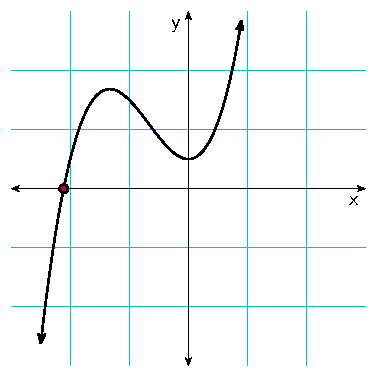
\includegraphics[scale=1]{polynomials/figures/cubic_with_one_real_root}
\caption{The real root of the cubic polynomial $f(x)=x^3+2x^2+0.5$}
\end{figure}

\section{Roots of Polynomials}
\begin{theorem}[Rational Root Theorem]
    If $P(x)$ is a polynomial with integer coefficients and $z=\frac{p}{q}$ is a 
    rational root, where $p$ and $q$ are in lowest terms, of $P(x)$ then 
    the leading coefficient, $a_{n}$, of $P(x)$ is a multiple of $p$ and the 
    constant term, $a_{0}$, of $P(x)$ is a multiple of $q$. 
\end{theorem}
\begin{corollary}
    If $P(x)$ is a polynomial with integer coefficients then every rational 
    root of $P(x)$ is an integer.
\end{corollary}

\section{Quadratic Polynomials}
\begin{definition}
    A \textit{quadratic polynomial} is a polynomial of the form,
    \[
        P(x) = ax^{2} + bx + c
    \]
    where $a,b,c$ are constants and $a\neq 0$.
\end{definition}
One can find the roots of a quadratic polynomial using the well known \textit{quadratic formula},
\[
    x_{1,2} = \frac{-b \pm \sqrt{b^{2} - 4ac}}{2a}
\]
The value $\Delta = b^{2} - 4ac$ is called the \textit{discriminant} of the quadratic polynomial. 
\begin{theorem}
    If $P(x)$ is some quadratic polynomial whose discriminant is $\Delta$ and 
    whose two roots are $x_{1}$ and $x_{2}$ then,
    \begin{itemize}
            \ii $\Delta>0 \iff x_{1}, x_{2} \in \mathbb{R} \text{ and } x_{1}\neq x_{2}$
            \ii $\Delta=0 \iff x_{1}, x_{2} \in \mathbb{R} \text{ and } x_{1}=x_{2}$
            \ii $\Delta<0 \iff x_{1}, x_{2} \in \mathbb{C} \text{ and } x_{1}\neq x_{2}$
    \end{itemize}
\end{theorem}

\begin{theorem}
    The value $P\left(-\frac{b}{2a}\right)$ is either the maximum (if $a>0$) or the minimum value (if $a<0$) of 
    the quadratic polynomial, $P(x)=ax^{2} + bx + c$
\end{theorem}
\begin{proof}
    \begin{align*}
                 P(x) &= ax^{2} + bx + c\\
        \implies P(x) &= a\left( x^{2} + 2\frac{b}{2a} x + \frac{b^{2}}{4a^{2}}\right) + c - \frac{b^{2}}{4a} \\
        \implies P(x) &= a\left(x + \frac{b}{2a}\right)^{2} + \left( c - \frac{b^{2}}{4a} \right)
    \end{align*}
    If $a<0$ then, 
    \[
        P(x) = \left( c - \frac{b^{2}}{4a}\right) - \abs{a}\left(x + \frac{b}{2a}\right)^{2}
    \]
    $P(x)$ will reach its maximum when $x + \frac{b}{2a} =0 \implies x = -\frac{b}{2a}$.\\
    If $a>0$ then,
    \[
        P(x) = \left( c - \frac{b^{2}}{4a}\right) + a\left(x + \frac{b}{2a}\right)^{2}
    \]
    $P(x)$ will reach its minimum when $x + \frac{b}{2a} =0 \implies x = -\frac{b}{2a}$.
\end{proof}

\begin{figure}[!htpb]
\begin{subfigure}[!htpb]{0.5\textwidth}
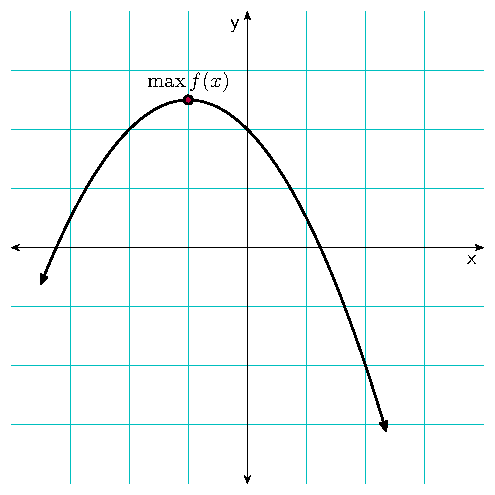
\includegraphics[scale=.85]{polynomials/figures/quad_max.pdf}
\caption{Maximum of $f(x)=-0.5x^2 - x + 2$}
\end{subfigure}
\begin{subfigure}[!htpb]{0.5\textwidth}
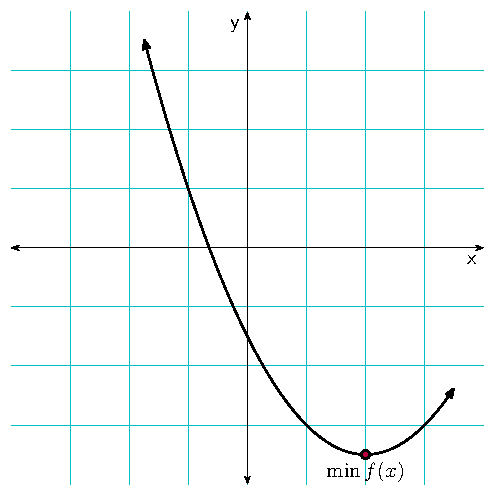
\includegraphics[scale=.85]{polynomials/figures/quad_min.pdf}
\caption{Minimum of $f(x)=0.5x^2 - 2x -1.5$}
\end{subfigure}
\end{figure}

\section{Lagrange Interpolation}

\begin{theorem}[Lagrange Interpolation]\label{thm:lagrange-interpol}
    Let $\alpha_{0}, \alpha_{1},\cdots , \alpha_{n}$ be distinct real numbers and 
    $\beta_{0}, \beta_{1}, \cdots, \beta_{n}$ be another set of $n+1$ real numbers. 
    Then there exists a unique polynomial,
    \[
    P(x) = \sum_{i=0}^{n} \left( \prod_{\substack{j=0\\ j\neq i}}^{n} \frac{x - \alpha_{j}}{\alpha_{i} - \alpha_{j}} \right) \beta_{i}
    \]
    with $\Deg P(x) \leq n$ such that $P(\alpha_{k}) = \beta_{k}$ for all $0\leq k \leq n$.
\end{theorem}
\begin{proof}
    Let,
    \[
    D_{k}(x) = \prod_{\substack{j=0 \\ j\neq k}}^{n} \frac{x - \alpha_{j}}{\alpha_{k} - \alpha_{j}} = 
    \frac{(x-\alpha_{0})(x-\alpha_{1})\cdots (x - \alpha_{k-1})(x - \alpha_{k+1}) \cdots (x - \alpha_{n})}
         {(\alpha_{k}-\alpha_{0})(\alpha_{k}-\alpha_{1})\cdots (\alpha_{k} - \alpha_{k-1})(\alpha_{k} - \alpha_{k+1}) \cdots (\alpha_{k} - \alpha_{n})}
    \]
    If $x=\alpha_k$ then $D_k(x) = 1$ else if $x=\alpha_i$ where 
    $i \neq k$ then $D_k(x)=0$. Thus the polynomial,
    \[ P(x) = \sum_{k=0}^n D_k(x) \beta_k \]
    will be equal to $\beta_k$ for all $x=\alpha_k$. It is also clear that the 
    polynomial $P(x)$ has degree at most $n$ since $\Deg D_k(x)=n$ for all 
    $0 \leq k \leq n$. \\
    Now suppose that there exists two polynomials $P_1(x)$ and $P_2(x)$, with degree at 
    most $n$, such that,
    \[ P_1(\alpha_k) = P_2(\alpha_k) = \beta_k, \; 0\leq k \leq n\]
    Therefore the polynomial $Q(x) = P_1(x) - P_2(x)$ has $n+1$ distinct roots. 
    But that is impossible since we know that $\Deg Q(x) \leq n$ and 
    a polynomial of degree $n$ has at most $n$ distinct roots. This proves that 
    the polynomial $P(x)$ must be unique, that is, $P(x)$ is the only polynomial, with 
    degree at most $n$, such that, 
    $P(\alpha_k) = \beta_k$ for all $0 \leq k \leq n$
\end{proof}

\begin{figure}[!htpb]
\centering
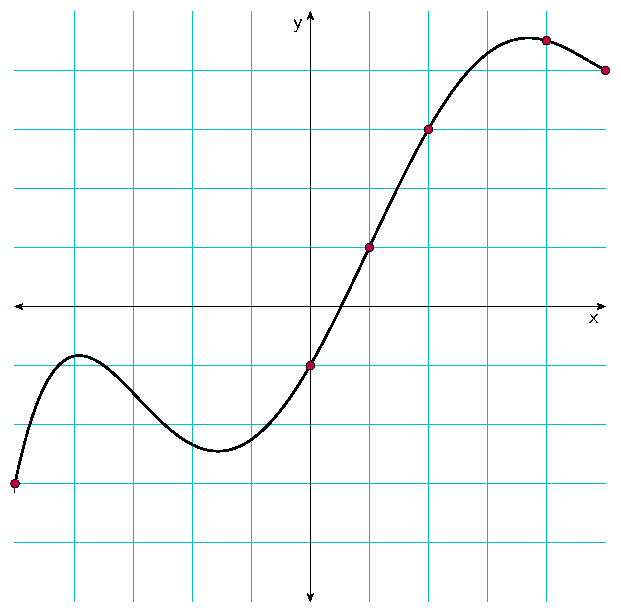
\includegraphics[scale=0.75]{polynomials/figures/lagrange_poly_plot1.pdf}
\caption{Plot of a Lagrange Polynomial}
\label{fig:lagrange_poly_plot1}
\end{figure}

\hyperref[fig:lagrange_poly_plot1]{Figure \ref{fig:lagrange_poly_plot1}} shows the Lagrange polynomial going through 
the points, 
\[ \left\{(1,1), (2,3), (0, -1), (5, 4), (-5, -3), (4, 4.5) \right\}\] 
We can easily compute Lagrange polynomials in python using \texttt{sympy}.

\begin{mdcode}
\begin{minted}[mathescape, breaklines, ]{pycon}
>>> import sympy
>>> x = sympy.symbols('x')
>>> points = [(1,1), (2,3), (0, -1), (5, 4), (-5, -3), (4, 4.5)]
>>> expr = sympy.interpolate(points, x)
>>> print(expr)
0.00281746031746032*x**5 - 0.0129761904761905*x**4 - 0.111944444444445*x**3 + 0.384404761904762*x**2 + 1.73769841269841*x - 1
\end{minted}
\end{mdcode}

\begin{problem}
    Let $P(x)$ be a polynomial of degree $n$ such that, $P(k)=2^{k}$ for all $0\leq k \leq n$. Find $P(n+1)$.
\end{problem}
\begin{sol}
    From \hyperref[thm:lagrange-interpol]{Theorem \ref{thm:lagrange-interpol}} we have,
    \begin{align*}
        P(x) = \sum_{k=0}^{n} 2^{k}D_{k}(x)
    \end{align*}
    where,
    \begin{align*}
        D_{k}(x) &= \frac{x(x-1)\cdots (x-k+1)(x-k-1)(x-k-2)\cdots (x-n+1)(x-n)}{(k)(k-1)\cdots (1)(-1)(-2) \cdots (k-n+1)(k-n)} \\
        &= (-1)^{n-k} \frac{x(x-1)\cdots (x-k+1)(x-k-1)(x-k-2)\cdots (x-n+1)(x-n)}{k!(n-k)!}
    \end{align*}
    Therefore,
    \begin{align*}
        P(n+1) &= \sum_{k=0}^{n} (-1)^{n-k} 2^{k} \frac{(n+1)n(n-1)\cdots (n-k+2)(n-k)(n-k-1)\cdots 1}{k!(n-k)!} \\
               &= \sum_{k=0}^{n} (-1)^{n-k} 2^{k} \frac{(n+1)!}{k!(n-k)!(n-k+1)} \\
               &= \sum_{k=0}^{n} (-1)^{n-k} 2^{k} {n+1 \choose k} \\
               &= (-1) \left( \sum_{k=0}^{n+1} {n+1 \choose k} 2^{k} (-1)^{n-k+1} \right) + 2^{n+1} \\
               &= (-1)\left( 2 - 1 \right)^{n+1} + 2^{n+1} \\
               &= 2^{n+1} - 1
    \end{align*}    
\end{sol}

